\documentclass[border=3pt]{standalone}
% Preâmbulo compartilhado pelos diagramas TikZ da aula 9 de IHR (Robôs na Sociedade)
\usepackage[T1]{fontenc}
\usepackage[utf8]{inputenc}
\usepackage{lmodern}
\usepackage{amsmath}
\usepackage{xcolor}
\usepackage{tikz}
\usetikzlibrary{arrows.meta,angles,quotes,decorations.pathmorphing,decorations.pathreplacing,calc,
                positioning,shapes.geometric,shapes.misc,backgrounds,fit,
                math}

% Paleta (mesma dos SVGs originais)
% Paleta da disciplina de IHR: acento azul (#1A6FB5), cor de destaque do tema.
% (o nome "dblue" é mantido para não alterar todos os diagramas)
\definecolor{dblue}{HTML}{1A6FB5}
\definecolor{dorange}{HTML}{B3541E}
\definecolor{dgreen}{HTML}{4A7C59}
\definecolor{dred}{HTML}{9C4B4B}
\definecolor{dcream}{HTML}{F4F1EA}
\definecolor{dshade}{HTML}{DDD7C9}

% Função gaussiana (não normalizada por padrão de escala visual)
\pgfmathdeclarefunction{gauss}{3}{%
  \pgfmathparse{1/(#3*sqrt(2*pi))*exp(-((#1-#2)^2)/(2*#3^2))}%
}

% Estilos comuns (prefixo d... para não colidir com chaves internas do pgf)
\tikzset{
  >={Stealth[length=2mm]},
  dguide/.style={gray!55, dashed, line width=0.4pt},
  daxis/.style={gray!60, line width=0.7pt, ->},
  dbody/.style={fill=black!3, draw=black!80, line width=1pt},
  dacc/.style={draw=dblue, line width=1pt},
  dlbl/.style={black!55, font=\small},
  dsub/.style={black!45, font=\footnotesize},
  dstate/.style={circle, draw=black!80, fill=dcream, line width=1pt,
                 minimum size=17mm, font=\large, inner sep=1pt},
  dobs/.style={circle, draw=black!80, fill=dshade, line width=1pt,
               minimum size=14mm, font=\large, inner sep=1pt},
  dbox/.style={rounded corners=2pt, draw=black!80, fill=dcream, line width=1pt,
               align=center, inner sep=6pt},
  dop/.style={circle, draw=black!80, fill=white, line width=1pt,
              minimum size=6mm, inner sep=0pt, font=\small},
  dtrans/.style={->, dblue, line width=1pt},
  dmeas/.style={->, dorange, line width=1pt},
  dcurve/.style={line width=1pt, dblue},
  dcurveb/.style={line width=1.4pt, dorange},
}

\begin{document}
\hyphenpenalty=10000 \exhyphenpenalty=10000 \tolerance=9999 \emergencystretch=3em
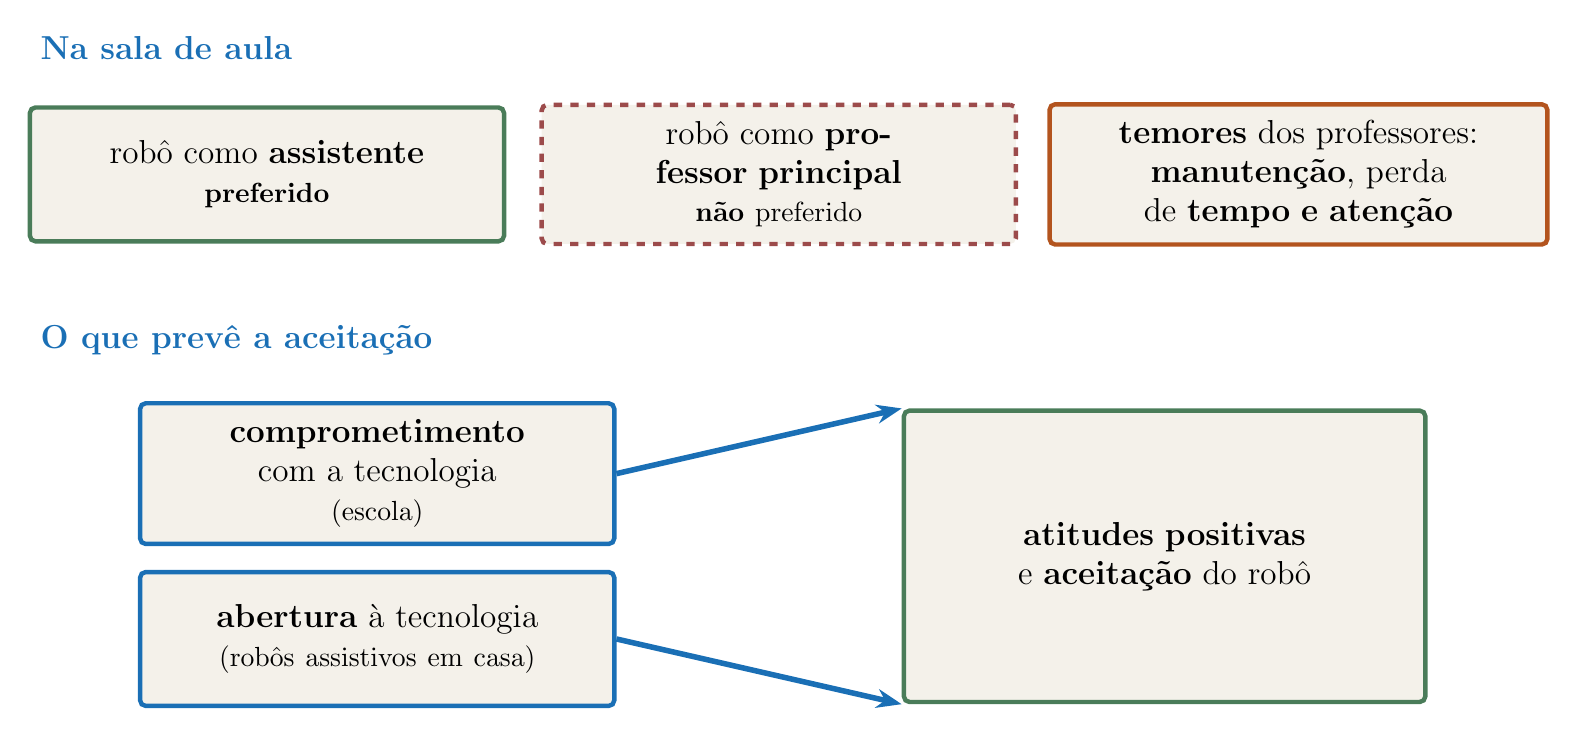
\begin{tikzpicture}[x=1cm,y=1cm]
\tikzset{k/.style={dbox, text width=5.6cm, minimum height=1.7cm, font=\large, line width=1.6pt}}
\node[font=\large\bfseries, dblue, anchor=west] at (0.2,8.4) {Na sala de aula};
\node[k, draw=dgreen] (a) at (3.2,6.8) {robô como \textbf{assistente}\\ {\normalsize \textbf{preferido}}};
\node[k, draw=dred, dashed] (b) at (9.7,6.8) {robô como \textbf{professor principal}\\ {\normalsize \textbf{não} preferido}};
\node[k, draw=dorange, text width=5.9cm] (c) at (16.3,6.8) {\textbf{temores} dos professores: \textbf{manutenção}, perda de \textbf{tempo e atenção}};
\node[font=\large\bfseries, dblue, anchor=west] at (0.2,4.7) {O que prevê a aceitação};
\node[k, draw=dblue] (d) at (4.6,3.0) {\textbf{comprometimento} com a tecnologia\\ {\normalsize (escola)}};
\node[k, draw=dblue] (e) at (4.6,0.9) {\textbf{abertura} à tecnologia\\ {\normalsize (robôs assistivos em casa)}};
\node[k, draw=dgreen, text width=6.2cm, minimum height=3.7cm] (f) at (14.6,1.95) {\textbf{atitudes positivas}\\ e \textbf{aceitação} do robô};
\draw[dtrans, line width=2pt, -{Stealth[length=3.2mm]}] (d.east) -- (f.north west);
\draw[dtrans, line width=2pt, -{Stealth[length=3.2mm]}] (e.east) -- (f.south west);
\end{tikzpicture}
\end{document}
